\subsection{Traitement audiovisuel}

Les tâches qui peuvent être automatisées sur une vidéo sont multiples : reconnaissance de locuteurs, segmentation audio, reconnaissance de visages, identification et classification d'objets, transcription audio, transcription de textes... Nous nous concentrons ici sur la segmentation temporelle, nous l'avons dit, c'est-à-dire sur la manière dont on peut automatiser la division d'une vidéo en différentes séquences, à partir de l'image et non du son. Nous analyserons ainsi les projets effectués dans ce domaine. Nos recherches ont montré que les études sur le sujet restent cantonnées aux expérimentations scientifiques et qu'elles n'ont pa été appliquées, à notre connaissance au domaine des humanités numériques. Nous établirons aini un état des lieux de ces expérimentations, afin de proposer la mise en place d'un tel processus en contexte patrimonial. 
on veut faire deux choses : segmenter les séquences et les décrire : mots-clés, classification... 

Les chercheurs qui analysent les objets visuels s'attachent de plus en plus à l'analyse vidéo car la détection du mouvement aide d'autres tâches d'analyse automatique de détection et de reconnaissance d'objets.  \footcite{brostow2009}
Les technologies appliquées à l'analyse de contenus vidéo et audio, comprenant la computer vision et la reconnaissance de discours automatique (ASR) sont désignées sous le terme de Audiovisual Processing (AVP). \footcite{noord2021}
aussi désigné sous les termes suivants : Audiovisual Processing technologies, Automatic Metadata Extraction, Metadata Generation Mechanisms, Machine Learning Applications for Visual/Audio Data Annotation.
 
De plus, les outils de traitement audiovisuel, appliqués à un grand nombre de données permettent de passer du "close" au "distant" viewing. \footcite{noord2021} En effet, au lieu d'analyser quelques archives audiovisuelles de manière isolée, les chercheurs/archivistes auraient l'opportunité d'obtenir une vue d'ensemble sur les données et d'en observer les tendances. L'application du traitement audiovisuel permet donc de changer notre rapport aux archives audiovisuelles. 

\subsubsection{Machine learning et deep learning}

Passage de l'analyse descriptive, à l'analyse prédictive : (computer vision > machine learning)
L'analyse predictive est plutot bien adaptée à l'audiovisuel 

Ces technologies reposent sur le machine learning, l'apprentissage machine, qui désigne un domaine de l'intelligence artificielle regroupant les techniques, méthodes et processus nécessaires afin de rendre une machine ou un système informatique plus intelligent. \footcite{zotero-item-584} Le machine learning désigne donc l'entraînement d'une machine à pouvoir "raisonner" à partir d'un jeu de données. Les techniques de traitement audiovisuels auraient ainsi besoin d'être entrainées sur des données, ici patrimoniales, afin de produire une analyse pertinente. 

Les technologies de traitement audiovisuel utilisent pour la plupart, une méthoe d'apprentissage machine, celle de l'apprentissge profond, fondée sur la mise en place de réseaux de neurones en pluieurs couches. Mais cette méthode requiert un nombre de paramètres important et un large jeu de données d'entraînement. \footcite{pattichis2023}

Pourquoi le deep learning ?

Analyse descriptive : 
définit un modèle mathématique qui décrit le phénomène à observer. Hypothèses formulées selon les tendances observées sur les données et validation de ces hypothèses en les comparant avec les résultats réels. mais modèle risqué car dépend des analyses humaines : oublis possibles, dépend des connaissances de celui qui fait les hypothèses, impossible de tout observer et tout prédire. \footcite{mahony2020}

Analyse prédictive : 
modèle qui minimise l'écart entre le résultat réel et le résultat prédit. Le machine learning fait de l'analyse prédictive. \footcite{mahony2020}

le deep learning est basé ur des réseaux de neurones artificiels inspirés du fonctionnement du cerveau humain. Les neurones sont en réalité des cellules de calcul qi interagissent les uns avec les utres afin de prendre uen décision. L'apprentissage profond permet à une machine d'apprendre à travers différentes couches de neurones sans supervisins humaine. Il suscite un intérêt croissant puisque l'interaction entre les cellules de calcul permettent une meilleure adaptabilité aux données. \footcite{mahony2020} Cette méthode d'apprentissage améliore aussi le rapport cout-efficacité. Les réseaux de neurones (CNN) sont entraînés plutot que programmés. Nécessitent moins de réglages et d'analyses humaine et grande flexibilité. les algorithmes de vision par ordinateur sont plus spécifiques à un domaine particulier. \footcite{mahony2020}

La vision par ordinateur est davantage utilisée pour décrire des caractéristiques à partir de la détection d'objets, et ainsi faire de la classification d'images. Mais il faut choisir en amont quelles caractéristiques l'algorithme doit choisir dans l'image. S'il y a beaucoup de caractéristques à extraire, le processus devient fastidieux et demande beaucou de supervision. Avec le deep learning, on fournit seulement quelques images annotées et les réseaux de neurones repèrent eux-mêmes les caractéristiques à extraire par rapport aux obejts observés.\footcite{mahony2020}

% TODO: \usepackage{graphicx} required
\begin{figure}
	\centering
	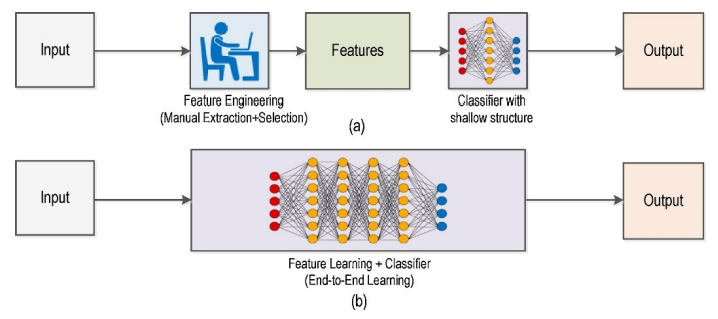
\includegraphics[width=0.7\linewidth]{images/screenshot001}
	\caption{mahony2020}
	\label{fig:screenshot001}
\end{figure}


Par rapport aux technique traditionnelles de vision par ordinateur, le deep learning permet d'avoir une plus grande précision dans les tâches d'analyse audiovisuelle telles que la classification d'images, la segmentation, le détection d'objets. \footcite{mahony2020}
risque des CNN : surapprentissage, difficle de modifier les paramètre uen fois qu'il est entraîné car miliers de paramètres entremêlés entre les cellecules de calcul. boite noires \footcite{mahony2020}
l'apprentissage automatique clasique, computer vision : transparence, les paramètres peuvent être ajustés manuellement et facilement. \footcite{mahony2020}

Les approches hybrides : un algorithme de vision par ordinateur peut détecter des caractéristiques qui peuvent ensuite être transmies à des réseaux de neurones profonds pour la classification. 

Mais tout dépend de la tâche à effectuer : peut être effectué à partir de la computer vision si c'est juste un seuil à calculer.

Les modèles multimodaux qui combinent audio et vidéo (vivit-ast) ne donnent pas les meilleurs résultats. Il faudrait donc adopter des architectures plus simples, qui demandent moins de calcul d'usage et qui séparent les pipelines. \footcite{attard2025}

Dans le deep learning : comparer les CNN et les transformers : 

CNN :  réseau de neurones convolutif 

Outils de classification : 
"modèles de programmation puissants permettant notamment la reconnaissance d’images en attribuant automatiquement à chaque image fournie en entrée, une étiquette correspondant à sa classe d’appartenance."\footcite{robert2026}
l'un des principaux cas d'usages des CNN est la "reconnaissance d'images". "Dans une moindre mesure, on les utilise aussi pour l’analyse vidéo.". \footcite{robert2026}

Description du fonctionnement d'un CNN appliqué à un corpus d'images : « CNNs learn a hierarchy of filters, which are applied to an input image in order to extract meaningful information from the input. [...] CNNs tend to learn features that resemble Gabor-like edge detectors and color-opponent filters at lower layers [...]. On higher layers of the CNNs, features capture more abstract image content by integrating the lower-layer features. » \footcite{brachmann2017}. A relier avec ResNet : même fonctionnement. 

limite des CNN pour l'analyse de l'esthétisme des images : « While hand-crafted features allow to quantify which feature contributes the most to an aesthetic rating, this interpretability is lost with generic features. [...] Deep neural networks and generic features basically represent a black-box approach that lacks this kind of interpretability. » \footcite{brachmann2017}

Transformer : 

"La fonctionnalité centrale des modèles transformers est leur mécanisme d’auto-attention, dont ils tirent leur incroyable capacité à détecter les relations (ou dépendances) entre les différentes partie d’une entrée. Contrairement aux architectures RNN et CNN qui l’ont précédée, l’architecture de type transformer utilise uniquement des couches d’attention et des couches de propagation standard." \footcite{bergmann2025}
Les RNN et CNN analyse les données de façon "sérielle" \footcite{bergmann2025}, dans un ordre donné, les empêchant ainsi de saisir les "dépendances à longue portée". \footcite{bergmann2025}
les tranformers : "Les mécanismes d’attention, quant à eux, examinent simultanément les séquences dans leur intégralité et décident de la manière et du moment où il convient de se concentrer sur certaines étapes de chaque séquence.", "En plus d’améliorer considérablement la capacité à comprendre les dépendances à longue portée, cette qualité des transformeurs permet également la parallélisation, qui consiste à réaliser plusieurs étapes de calcul simultanément, au lieu de les sérialiser." \footcite{bergmann2025}

"Les transformeurs offrent également certains avantages par rapport aux réseaux de neurones, en particulier pour les données visuelles. Intrinsèquement locaux, les CNN utilisent des convolutions pour traiter successivement les sous-ensembles de données d’entrée.
Par conséquent, les CNN peinent à discerner les dépendances à longue portée, telles que les corrélations entre les mots (dans un texte) ou les pixels (dans une image) qui ne sont pas voisins. Les mécanismes d’attention n’ont pas cette limitation." \footcite{bergmann2025}

Les modèles fondés sur les mécanismes d'auto attention capturent mieux les relations entre images mais leur complexité les rend difficilement applicables à des vidéos complexes elles mêmes.\footcite{yuan2025}

segmentation sémantique vidéo adaptative TDNet et TDSNet 
low parameter models 

outils : 
shot boundary detection : pyscene detect, 2SDS + amaliajs
framework de computer vision : diginpix, detectron, imageJ
modèles d'action reconigtion standards : TSN, slowfast


transition vers la prochaine sous partie : parler des données d'entrainement (cf fichier IAvideo pattichis)

Toutes les tâches automatiques qui peuvent être appliquées à la vidéo nécessitent un entraînement multimodal : 
entrainemen multimodal :  When we refer to multimodal or cross-modal learning, we are referring to learning using video, audio and/or text. These approaches generalize to a greater variety of visual tasks including action step localization, action segmentation, text-to-video retrieval, video captioning. \footcite{schiappa2023}


\subsubsection{outils et modèles disponibles}
Analyse sémantique vs analyse syntaxique : 

citer diginpix 

La détection de coupures = analyse syntaxique et ne nécessite pas de réseaux de neurones aux calculs lourds 
appliquer plutot 2sds ou pyscenedetect : étapes 

mais : identifier et classifier la séquence, le décrire (shot semantics) : avec l'apprentissage supervisé avec signgle shot detectors  (classer le type de plans, le type d'objets...)
deux voies pour décrire séquence : 
par keyframes (vitesse) Diginpix
par densité temporelle (précision) TDSNet

zero shot learning pour la description : CLIP 

Malgré de grandes avancées dans le processing audiovisuel, avec des outils comme la computer vision appliquée à la vidéo, et la reconnaissance de discours automatique (ASR), ces outils restent largement inaccessibles et hors de portée pour les institutions patrimoniales. \footcite{noord2021}. Ils sont utilisés par des entreprises commerciales pour du montage vidéo par exemple. Le manque d'utilisation de ces outils dans le domaine des sciences humaines expliquent l'inexistance de données d'entraînement adaptées au secteur. \footcite{noord2021} 
l'analyse vidéo par un processus humain prend un temps considérable, puiqu'il faut lire le fichier audiovisuel et en analyser les composants, le langage. Ainsi, l'indexation des archives audiovisuelles se cantonne souvent aux métadonnées, sans en exposer les données, le contenu.

Et donc en pratique, comment appliquer le traitement audiovisuel à des corpus d'archives audiovisuelles patrimoniales ? 

pipeline avec 2SDS : 
\subitem 2SDS

l'étude de xin2023 \footcite{xin2023} présente 2SDS, un algorithme de segmentation temporelle vidéo. Plutôt que d’utiliser un réseau de neurones pour détecter les changements de scènes, 2SDS compare des empreintes (hash) d’images successives. Si deux frames sont suffisamment différentes (distance de Hamming supérieure à un seuil), elles appartiennent à des scènes distinctes.
« 2D CNNs only recognise a video as discrete images, rather than a continuous stream of images. This poses some issues. For example, a CNN model could not resolve the motion of a person because the person is stationary in every frame, and this will cause the loss of significant information in video analysis. »\footcite{xin2023} : un CNN 2D comme resnet analyse chaque plan de manière indépendante et ignore la logique temporelle de la vidéo. 2SDS résout ce problème en regroupant les plans similaires avant de les classifier. (à relier avec la notion de shot boundary detection). 
« We need to devise an implementation that complements the CNN model to solve the continuity issue. This implementation should group the discrete frames (adjacent on the temporal axis) that look similar to each other into scenes, this procedure is what we call temporal segmentation. »\footcite{xin2023} : la segmentation temporelle : regrouper les plans qui se suivent et visuellement similaires : c'est ce que fait pyscene detect avec le content detector. 
l'article explique aussi la mise en place d'un pipeline de détection de changement de plan : 
4 étapes : 
\subitem down sampling : miniaturisation du plan pour détecter les changements globaux, pas locaux
\subitem conversion de l'image RGB en niveaux de gris 
\subitem calcul d'une valeur de "hachage" de l'image : Chaque ligne de 9 pixels est convertie en 8 bits binaires comparant les pixels adjacents. Produit une « empreinte » numérique de la frame.
\subitem distance de hamming : 
comparaison des empreinte de deux frames consécutives. Si la distance est supérieure à 5, les deux plans apparatiennent à des scènes différentes. le seuil est paramétrable. pyscenedetect est l'implémentation concrète de ce processus. 

les auteurs conseillent de ne pas utiliser des réseaux de neurones pour la segmentation vidéo : « The usage of RNN or even neural networks is not practical in time sensitive tasks like real-time object recognition and live video stream analysis, which requires fast responding algorithms, and RNNs usually cannot meet those requirements. »\footcite{xin2023}

détecter les coupures entre es scènes est une analyse syntaxique et non sémantique : il suffit de détecter la différence visuelle. les meilleurs résutats de détection de coupures se font sur des plans fixes, avec des suets distants, des mouvements lents, docn plutot bien adaptées aux archives audiovisuelles. 

l'article de \cite{xin2023} ne cherche pas à comprendre les scènes mais seulement à analyser leur syntaxe pour en détecter les coupures. 2SDS règle le problème de délimitation en séquence, mais ne décrit pas la vidéo comme d'autres outils peuvent le faire : CLIP, YOLO, BLIP. De plus, le corpus de tets ets réduit (6 vidéos issues de youtube), et en couleur. 


 pipeline multimodal 
Automatic temporal vidéo scene segmentation (ou video story segmentation)

"The automatic temporal video scene segmentation (also known as video story segmentation) is still an open problem without definite solutions in most cases." \footcite{trojahn2021}
les meilleurs solutions et qui donnent les meilleurs résultats qui existent sont les techniques mutlimodales utilisant les caractérstiques de plusieurs outils : "Among the available techniques, the ones which shows better results are multimodal using features extracted from multiple modalities."\footcite{trojahn2021}
La fusion multimodale peut se faire de deux façon, fusion en une seule représentation, fusion par segmentation de chaque modalité : "Multimodal fusion may be performed to fuse each modality as a single representation (early fusion) or by each modality segmentation (late fusion), the latter been widely due to multimodal fusion simplicity."\footcite{trojahn2021}. C'est la seconde approche qui est privilégiée. 

limites des CNN : "CNNs cannot adequately learn cues which are temporally distributed along the video due to difficulties to model temporal features data dependencies."\footcite{trojahn2021}

RNNs : "Successfully employed on text processing, RNNs are fitted to analyze sequences of data of variable length and may better grasp the temporal relationship among low-level features of video segments, hopefully obtaining more accurate scene boundary detection."\footcite{trojahn2021}. Les RNN permettent de mieux capturer les relations temporelles. 

Une des solutions serait de combiner CNN et RNN : complémentaires.

La segmentation en pratique (Le cas du corpus Albert Kahn  DigInPix) : Pour analyser ce corpus, la première tâche est de briser le flux vidéo en unités distinctes appelées shots (plans) (Arnold  Tilton, 2019). C'est ici que vous intégrez le fonctionnement de DigInPix (développé par l'INA pour les images fixes et animées) : pour gérer la dimension temporelle, le système extrait des keyframes (images clés) dès que le contenu change significativement (nouveau plan, mouvement de caméra, nouvel objet) grâce à des histogrammes basés sur les descripteurs LBP (Local Binary Patterns) (Letessier et al., 2015). Une fois ces unités analysables isolées, on peut y appliquer de la reconnaissance (visages, objets) (Arnold  Tilton, 2019 ; Letessier et al., 2015).

segmentation spatiale, temporelle, sémantique, audio

ex du corpus albert kahn 

\subsubsection{entraîner ces outils et ces modèles}

les modèles de détection neuronaux sont entrainés sur des datasets de clips courts. Or, la réalité auiovisuelle est bien différente. \footcite{pattichis2023} Des approches algorithmiques non neuronales ou hybrides seraient donc plus adaptées car fondée sur des calculs et des seuils matéhmatiques : plus stable. 

détection des coupures : 
approche algorithmique non neuronale (2SDS, pyscenedetect), (xin et attard) pipeline technique en 4 étapes (down sampling (miniaturisation), conversion en niveaux de gris, calcul d'empreinte numérique par hachage binaire des pixels, et calcul de la distance de Hamming pour marquer la rupture visuelle (xin2023)

efficace sur les plans fixes et mvts lents 

mettre en rapport avec les travaux d'Arnold  Tilton (2019), qui utilisent une méthode similaire combinant différences d'histogrammes et réduction de résolution des pixels (downsampling) pour mesurer les ruptures de palettes de couleurs et de luminosité d'une frame à l'autre, complétée par des règles logiques pour éviter les faux positifs lors des fondus (fade-in/fade-out).

L'apport de l'IA (Vers la classification sémantique) : La détection brute des coupures ne suffit plus ; l'enjeu actuel est la Shot semantics (décrire le contenu d'un plan et sa typologie) (Arnold  Tilton, 2019).

Le rôle des modèles (CNN et Détecteurs) : Pour analyser le contenu de ces plans, on utilise l'apprentissage supervisé (Supervised Learning), où des algorithmes apprennent à partir de données labellisées par l'humain (DeLua, 2024). C'est le cas des réseaux de neurones convolutifs (CNN) comme Faster R-CNN ou YOLO (un détecteur de type Single Shot qui prédit et classifie "en une seule fois") pour la détection d'objets ou de visages (Arnold  Tilton, 2019 ; Robert, 2026).

Le méta-algorithme de classification : Arnold  Tilton (2019) montrent qu'en combinant la position des visages détectés et les coupures de plans, on peut créer un méta-algorithme capable de classifier automatiquement le type de plan (gros plan/close-up, plan amorce/over the shoulder), permettant de comprendre comment le cadrage construit le récit.

\subsubsection{analyse du mouvement}

au lieu d'utiliser des larges modèles qui tentent de tout classifier, plutot utiliser des modèles "low parameter", c'est-à-dire des modèles 3D-CNN légers, avec moins de paramètres dédiés à la reconnaissance d'une seule activité précise. prenennt moins de mémoire vidéo. \footcite{pattichis2023}

stratégie de réduction de l'annotation humaine : slf supervised learning, semi supervised, active learning, zero shot \footcite{pattichis2023}

confronter les architectures de réseaux de neurones (CNN vs. Transformers), introduire l'apprentissage non supervisé (Unsupervised Learning / DeepCluster),

Les limites des CNN 2D classiques (comme ResNet) : ils analysent la vidéo comme des images discrètes et indépendantes, ignorant la continuité du mouvement \footcite{xin2023}. Se tourner vers les vision transformers : CLIP, ViViT (bergmann et al), mécanismes d'auto attention qui analysent l'intégralité d'une séquence

Les modèles de Video Semantic Segmentation (VSS) et le dilemme entre les méthodes orientées "vitesse" (approche par keyframes peu précise) et orientées "précision" (TDNet, flux optique, mécanismes d'auto-attention) \footcite{zhou2022}.

La gestion du coût de calcul : présentation de TDSNet (TFRM pour extraire les zones dynamiques par soustraction d'images consécutives, et MMRM pour pondérer selon la magnitude réelle du mouvement) \footcite{yuan2025}. règle ce dilemme 

alternatives non supervisées : la supervision demande des données annotées (caron et al), l'apprentissage non supervisé (Unsupervised Learning) comme DeepCluster (Caron et al., 2018). Ce type de modèle regroupe les images ou frames similaires en "clusters" algorithmiques (via K-means) pour s'auto-entraîner sans intervention humaine (Caron et al., 2018). Si DeepCluster s'avère robuste face à des changements de distribution d'images (ce qui est prometteur pour des archives spécifiques), il présente deux limites majeures : il introduit des biais imprévisibles en remplaçant les labels par des métadonnées brutes (inacceptable pour la rigueur historienne) et a été conçu sur des bases gigantesques (ImageNet, 1.28 million d'images), le rendant difficilement transposable à des collections d'archives réduites (Caron et al., 2018 ; Norindr, 2023).

infrastructure locale : amener l'algorithme aux données : C'est la discussion centrale de votre partie. Les outils d'AVP commerciaux (souvent basés sur le Cloud) sont inutilisables pour les archives en raison des droits de propriété intellectuelle et de la sécurité des données (van Noord et al., 2021). La solution réside dans des architectures locales comme DANE (projet CLARIAH), basées sur un système décentralisé de workers (van Noord et al., 2021). Ce type d'infrastructure produit des métadonnées exploitables, mais aussi des vecteurs de caractéristiques (représentations abstraites) ouvrant la voie à la recherche par similarité visuelle ou sonore (van Noord et al., 2021).

La note finale sur l'explosion des données : L'indexation automatique par IA (comme avec DigInPix ou les modèles de type VLM) génère une masse d'informations locales phénoménale : les bases de données constituées peuvent être plus lourdes en taille que les fichiers vidéos d'origine (Moiraghi  Letessier, 2018).

transition : nécessité d'un mapping vers le FRBR : faire correspondre la sortie de ces pipelines avec un modèle de données. 